\documentclass[11pt]{article}
\usepackage[a4paper,margin=1in]{geometry}
\usepackage[T1]{fontenc}
\usepackage[utf8]{inputenc}
\usepackage{lmodern}
\usepackage{microtype}
\usepackage{amsmath,amssymb}
\usepackage{booktabs}
\usepackage{multirow}
\usepackage{graphicx}
\usepackage{xcolor}
\usepackage{hyperref}
\hypersetup{colorlinks=true,linkcolor=black,citecolor=blue,urlcolor=blue,
  pdftitle={Deriving, Testing, and Bounding the Multi-Power Law for Loss-Curve Prediction},
  pdfauthor={Jiaju Wu}}
\usepackage{titlesec}
\titlespacing*{\section}{0pt}{10pt}{4pt}
\titlespacing*{\subsection}{0pt}{6pt}{2pt}
\titlespacing*{\paragraph}{0pt}{4pt}{6pt}

\newcommand{\code}[1]{\texttt{\small #1}}

\title{\vspace{-2.2em}\textbf{Deriving, Testing, and Bounding the Multi-Power Law\\
for Schedule-Aware Loss-Curve Prediction}}
\author{Jiaju Wu \quad (Student ID: 2400010711)\\
\small Code: \url{https://github.com/wjjpku/DL-final}}
\date{}

\begin{document}
\maketitle

\begin{abstract}\noindent
Predicting how the pretraining loss of a language model evolves under a given
learning-rate (LR) schedule lets researchers compare schedules \emph{before}
spending compute. We reproduce the two representative empirical laws---the
\emph{Scaling Law with LR Annealing} (Tissue et al.) and the \emph{Multi-Power
Law} (MPL, Luo et al.)---fitting on cosine schedules and predicting the unseen WSD
family across $25/100/400$M models, recovering their published accuracy. We then
study MPL from first principles. A derivation from SGD on a power-law curvature
spectrum gives each of MPL's parameters a physical identity and predicts that its
\emph{exponents} are set by the spectral shape (scale-invariant) while its
\emph{amplitudes} track the spectral scale; the data confirm this---the exponents
$\{C,\beta,\gamma\}$ vary by only $1\text{--}2\%$ over a $16\times$ range, and as a
consequence all $27$ curves collapse onto a single master power law
($R^2{=}0.997$). Guided by the theory we develop two methods to improve MPL---a
scale-conditioned variant and a new discrete-step $(S,Q)$ asymptotic---and report
honestly that MPL is near-optimal on these data, also showing how an
under-optimized baseline can fabricate an apparent win. Finally we resolve MPL's
one purely empirical parameter, the LR-modulation exponent $\gamma$: it is
essential on real data ($3\text{--}4\times$ worse without it) yet provably absent
from any spectral quadratic-SGD model. We localize it to the non-linear
\emph{edge of stability} ($\eta\lambda\!\sim\!1$), explaining why it can only be
fit, not derived.
\end{abstract}

\section{Problem and Motivation}
Pretraining large language models is expensive, and the LR schedule shapes the
entire loss trajectory~\cite{kaplan2020,hoffmann2022,hu2024minicpm}. Classical
scaling laws predict a single end-of-training loss from model size $N$ and data
$D$; they are silent about how the loss \emph{curve} responds to the \emph{shape}
of the schedule (warmup, decay form, horizon). \emph{Schedule-aware loss-curve
prediction} closes this gap: given $\{\eta_t\}$, predict $L(t)$. This replaces
trial pretraining runs with a formula, exposes mid-training dynamics, and once it
extrapolates to unseen schedules can be inverted to \emph{search} for better
ones~\cite{luo2025}. The defining test is cross-schedule generalization: fit on
cosine, predict the unseen WSD family. We reproduce this and then ask a sharper
question---can the governing law be \emph{derived}, \emph{improved}, and its
\emph{limits} pinned down?---answered as one study on public curves at three
scales.

\section{Background: Two Empirical Laws}
Write $S(t)=\sum_{i\le t}\eta_i$ for the cumulative LR (a natural ``time''), and
$\Delta\eta_k=\eta_{k-1}-\eta_k$ for the LR decrement at step $k$.
\emph{Tissue et al.} (5 params): $L=L_0+A\,S^{-\alpha}-C\,S_2$, with $S_2$ a
momentum-smoothed annealing area; simple but coarse.
\emph{Multi-Power Law} (7 params):
\begin{equation}\label{eq:mpl}
L(t)=L_0+A\,S(t)^{-\alpha}+B\!\sum_{k\le t}\!\Delta\eta_k\,
G\!\big(\eta_k^{-\gamma}(S(t)-S(k))\big),\quad G(x)=1-(1+Cx)^{-\beta}.
\end{equation}
The sum ($LD$) models how each LR decrease keeps reducing the loss. MPL is the
state of the art; the factor $\eta_k^{-\gamma}$ is fit empirically---a point we
resolve in \S\ref{sec:eos}.

\section{Experimental Reproduction}\label{sec:repro}
We use the official public loss curves (Llama-2-style models at $25/100/400$M,
$9$ schedules each), fit on cosine schedules, and evaluate on the five unseen
WSD-family curves. Both laws are fit by minimizing a Huber loss on $\log L$ with
L-BFGS-B and multi-start (Tissue's $S_2$ rewritten as an exact linear recurrence;
MPL's $LD$ vectorized). Table~\ref{tab:repro} and Fig.~\ref{fig:1}a recover the
published behavior: MPL is more accurate at $25/400$M and ties Tissue at $100$M,
and our MPL test MAE ($0.0054/0.0050/0.0085$) matches Luo et al. This well-fit MPL
is the baseline the rest of the paper respects.

\begin{table}[t]\centering\small
\caption{Reproduction: average test MAE on WSD curves (fit on cosine).}
\label{tab:repro}
\begin{tabular}{lccc}
\toprule
Scale & Tissue (5p) & MPL (7p) & Better \\
\midrule
25M  & 0.00783 & \textbf{0.00539} & MPL (5/5 curves)\\
100M & \textbf{0.00486} & 0.00496 & tie\\
400M & 0.00979 & \textbf{0.00852} & MPL (5/5 curves)\\
\bottomrule
\end{tabular}
\end{table}

\begin{figure}[t]\centering
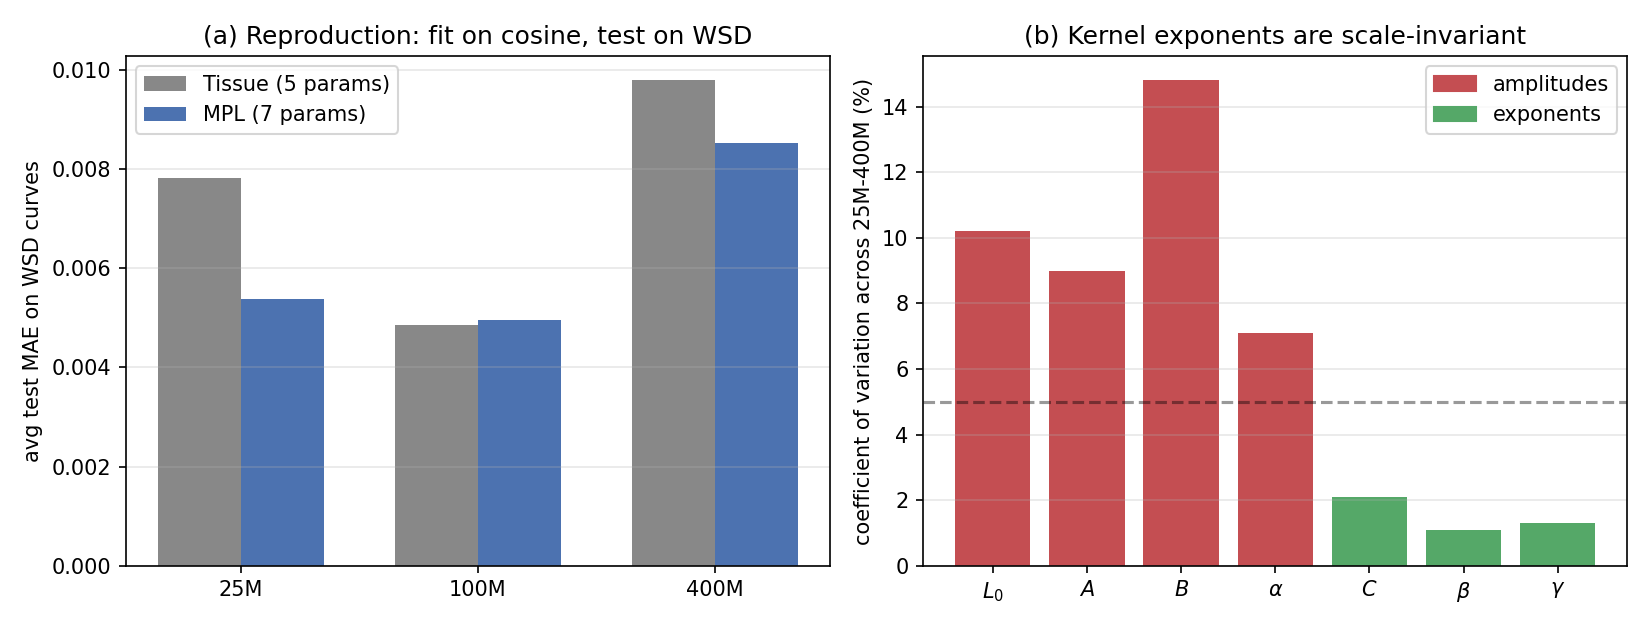
\includegraphics[width=0.92\linewidth]{figs/fig1_repro_invariance.png}
\caption{(a) Reproduction of Tissue vs.\ MPL (cosine$\to$WSD).
(b) The kernel \emph{exponents} $\{C,\beta,\gamma\}$ vary by $1\text{--}2\%$ across
$16\times$ scale; the \emph{amplitudes} $\{L_0,A,B\}$ and $\alpha$ by
$7\text{--}15\%$.}
\label{fig:1}
\end{figure}

\section{Deriving MPL from SGD Dynamics}\label{sec:theory}
MPL's seven parameters are accurate but opaque. We derive the form from a
tractable model, giving each parameter a physical identity and a prediction about
its scale dependence. This recovers and details the spectral picture sketched by
Luo et al.

\paragraph{Model.}
Near the trajectory the loss is locally quadratic; in the Hessian eigenbasis,
mode $i$ has curvature $\lambda_i$ and gradient-noise variance $\sigma_i^2$, and
SGD is the linear noisy recurrence
\begin{equation}\label{eq:rec}
\delta_i(t{+}1)=(1-\eta_t\lambda_i)\,\delta_i(t)-\eta_t\xi_i(t),\quad
L=L_{\min}+\tfrac12\textstyle\sum_i\lambda_i\,\mathbb E[\delta_i^2].
\end{equation}
For small steps $(1-\eta\lambda)\approx e^{-\eta\lambda}$. The second moment
splits into a deterministic bias and a stochastic noise floor.

\paragraph{Bias gives the power-law backbone.}
With $\delta_i^{\mathrm{bias}}\!\approx\!\delta_i(0)e^{-\lambda_i S}$ and bias
spectral density $g(\lambda)\sim c\lambda^{a}$, a Tauberian argument gives
\begin{equation}\label{eq:bias}
L_{\mathrm{bias}}(S)=\int_0^\infty\! g(\lambda)e^{-2\lambda S}d\lambda \;\sim\;
A\,S^{-\alpha},\qquad \alpha=a+1 ,
\end{equation}
with $L_0=L_{\min}$ the irreducible loss.

\paragraph{The noise floor gives the annealing term.}
Solving the variance recurrence and integrating in $S$,
$V_i(t)\!\approx\!\sigma_i^2\!\int_0^{S(t)}\!\eta(S')e^{-2\lambda_i(S(t)-S')}dS'$;
at constant LR the noise loss is $\propto\eta$ (the floor tracks the current LR).
The bonus from \emph{decaying} below the peak, written via the decrements, is
\begin{equation}\label{eq:conv}
\Delta N(t)=\sum_k\Delta\eta_k\,\mathcal K\!\big(S(t){-}S(k)\big),\quad
\mathcal K(y)=\!\int_0^y\!\!\!\int\! h(\lambda)e^{-2\lambda x}d\lambda\,dx ,
\end{equation}
\emph{exactly} MPL's $LD$ structure; a Gamma spectrum
$\propto\!\lambda^{\beta-1}e^{-\lambda/\lambda_0}$ makes
$\mathcal K(y)\!\propto\!1-(1+Cy)^{-\beta}$ with $C=2\lambda_0$, MPL's kernel.

\paragraph{What the derivation predicts.}
Collecting terms reproduces Eq.~\eqref{eq:mpl} (without $\eta_k^{-\gamma}$, see
\S\ref{sec:eos}) and, crucially, splits the parameters by origin:
$\{\alpha,\beta,C\}$ are functions of the spectral \emph{shape}
($a$, $\beta$, $\lambda_0$), whereas $\{L_0,A,B\}$ are set by the irreducible loss
and the spectral \emph{scale}. \textbf{Prediction:} if the curvature spectrum
keeps its shape as width $N$ grows, the exponents are scale-invariant and only
the amplitudes drift with $N$.

\section{Scale Invariance and a Universal Master Curve}\label{sec:invariance}
Fitting MPL per scale (Fig.~\ref{fig:1}b) confirms the prediction:
$C,\beta,\gamma$ have coefficient of variation $2.1\%,1.1\%,1.3\%$, while
$L_0,A,B$ drift by $9\text{--}15\%$ and $\alpha$ (an initialization-weighted
exponent, expected to be the least stable of the four) by $7\%$.

This has a striking consequence. Algebraically MPL is a \emph{single} power law
$L=L_0(N)+A(N)\,\tau^{-\alpha}$ in the effective progress
$\tau=[\,S^{-\alpha}+(B/A)LD\,]^{-1/\alpha}$, which folds the schedule's annealing
into one variable. Using \emph{one} shared exponent set
$\{\alpha^\ast,C^\ast,\beta^\ast,\gamma^\ast\}$ and only per-scale amplitudes, all
$27$ curves---$3$ scales $\times$ $9$ schedules---collapse onto the master curve
$y=\tau^{-\alpha}$ with $R^2{=}0.997$ (Fig.~\ref{fig:2}). The collapse succeeds
only because a single exponent set fits every scale, so it is a direct visual
proof of scale invariance: there is essentially \emph{one} loss curve, with model
size and schedule merely reparameterizing the axes.

\begin{figure}[t]\centering
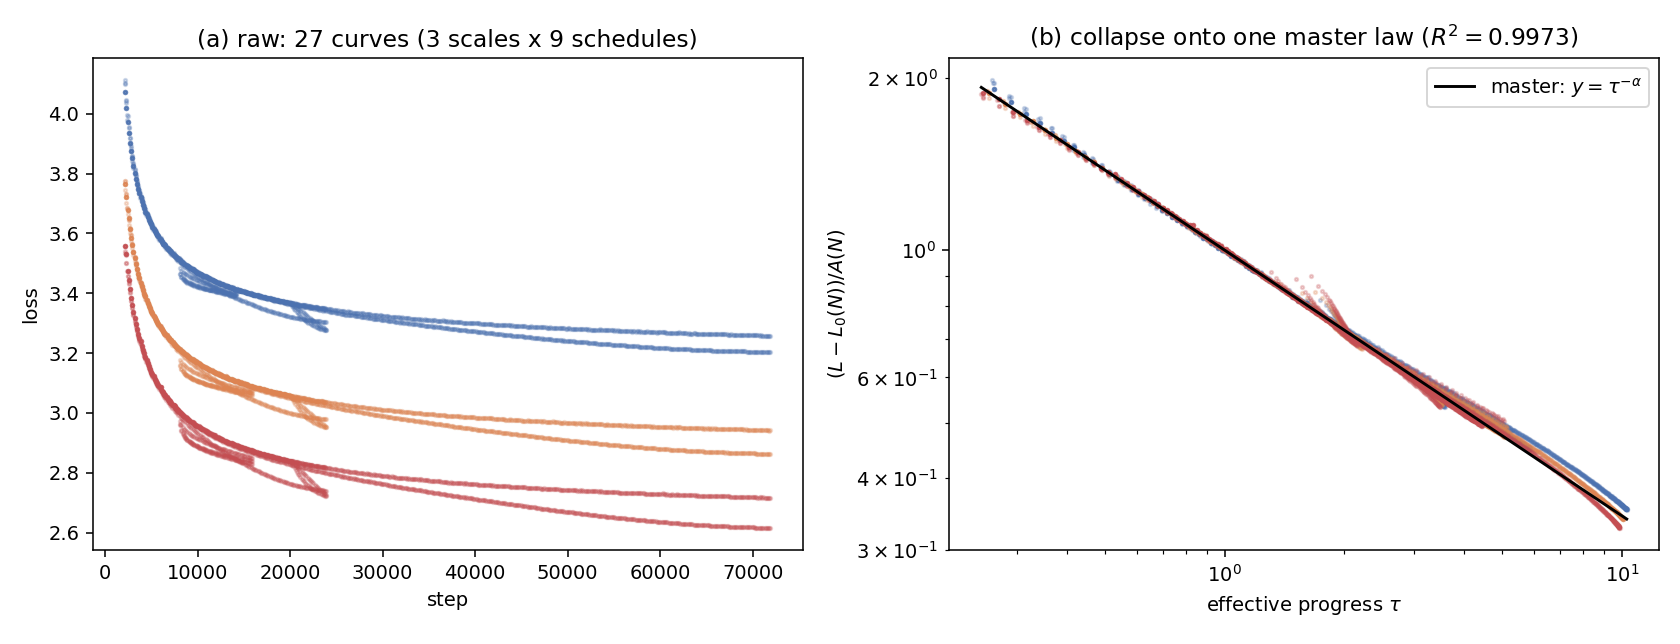
\includegraphics[width=0.99\linewidth]{figs/fig2_collapse.png}
\caption{(a) The $27$ raw loss curves (color = scale, $9$ schedules each).
(b) Under one scale-invariant effective-progress map $\tau$ and per-scale
amplitudes, they collapse onto a single master power law $y=\tau^{-\alpha}$
($R^2{=}0.997$).}
\label{fig:2}
\end{figure}

\section{Method Development: Two Attempts to Improve MPL}\label{sec:methods}
The derivation suggests two principled ways to do better than a $7$-parameter
per-scale fit. We report both honestly.

\paragraph{SC-MPL (scale-conditioned).}
Since the exponents are scale-invariant, we freeze $\{\alpha,C,\beta,\gamma\}$ at
values borrowed from cheaper small models and fit only the three amplitudes
$\{L_0,A,B\}$ on the target---cutting a new scale from $7$ free parameters to $3$.
Under a fair protocol (MPL uses its published, well-optimized parameters; SC-MPL
does only the stable amplitude fit) SC-MPL is competitive at $100$M (winning
$4/6$ curves with far fewer parameters) but does not beat a well-fit MPL at
$400$M (Table~\ref{tab:methods}, top): the residual drift, chiefly in $\alpha$,
costs more than the parameter economy gains. \emph{Caution:} an earlier protocol
that re-fit the MPL baseline into a poor optimum made SC-MPL look $20\%$ better;
giving the baseline its true optimum erases that ``win.''

\paragraph{Q-MPL (a new discrete-step asymptotic).}
Tissue and MPL both use the continuum approximation, leaving the single time
variable $S=\sum\eta$. Keeping the next discrete-step order introduces a
\emph{second} time variable $Q=\sum\eta^2$ (from
$\prod(1-\eta\lambda)^2\!\approx\!e^{-2\lambda S-\lambda^2 Q}$); expanding the
bias integral yields a derived correction $\propto Q\,S^{-(\alpha+2)}$. Testing
$\text{Q-MPL}=\text{MPL}+E\,Q\,S^{-(\alpha+2)}$ on cosine$\to$WSD
(Table~\ref{tab:methods}, bottom), the data drive $E\!\to\!0$ at $25/100$M (the
term is unnecessary) and, when free, over-fit the cosine train and worsen the WSD
prediction at $400$M. Q-MPL does not beat MPL.

\paragraph{Verdict.}
Two principled extensions fail to improve a well-fit MPL, and the universal
collapse shows MPL already captures essentially all reproducible structure. We
conclude, honestly, that MPL is near-optimal on these curves; the residual
($\text{MAE}\!\sim\!0.003$) carries no structure a derived correction exploits.
Beating it would likely require data exposing MPL's failure modes---more extreme
schedules or more scales---the natural data bottleneck of this study.

\begin{table}[t]\centering\small
\caption{Method development, fair comparisons (avg test MAE).
\emph{Top}: SC-MPL on the official split (MPL = published per-scale fit).
\emph{Bottom}: Q-MPL on cosine$\to$WSD.}
\label{tab:methods}
\begin{tabular}{llccc}
\toprule
 & Scale & MPL & SC-MPL-4 & SC-MPL-3 \\
\midrule
\multirow{2}{*}{SC-MPL}
 & 100M & \textbf{0.00435} & 0.00451 & 0.00525\\
 & 400M & \textbf{0.00484} & 0.00760 & 0.00786\\
\midrule
 & Scale & MPL (7p) & Q-MPL (8p) & $E^\ast$\\
\midrule
\multirow{3}{*}{Q-MPL}
 & 25M  & \textbf{0.00715} & 0.00715 & ${\approx}0$\\
 & 100M & \textbf{0.00386} & 0.00386 & ${\approx}0$\\
 & 400M & \textbf{0.00669} & 0.00824 & overfit\\
\bottomrule
\end{tabular}
\end{table}

\section{The Edge-of-Stability Origin of \texorpdfstring{$\gamma$}{gamma}}\label{sec:eos}
MPL's one purely empirical parameter is the LR-modulation exponent $\gamma$, which
our derivation does not produce. We show it is both \emph{essential} and
\emph{underivable from quadratic theory}, and localize its physical origin.

\paragraph{It is essential on real data.}
Holding all exponents at their fitted values and only setting $\gamma{=}0$ (then
re-fitting the amplitudes) inflates the test MAE by $3\text{--}4\times$
(Table~\ref{tab:gamma}, ``real''). The original authors were right to include it.

\paragraph{It cannot come from the quadratic model.}
Because $S$-units absorb $\eta$ in Eq.~\eqref{eq:conv}, the leading kernel has no
LR-magnitude factor: the theory predicts $\gamma{=}0$. The dependence hides one
order down, in the second time variable $Q=\sum\eta^2$, so $\gamma$ is a
sub-leading discrete-step effect. But the term $\lambda^2 Q$ matters only when
$\eta\lambda\!\sim\!1$---the highest-curvature modes, i.e.\ the \emph{edge of
stability}~\cite{cohen2021,damian2023}, where the linearized
recurrence~\eqref{eq:rec} diverges rather than relaxes. A deterministic mean-loss
simulation confirms it: fitting MPL and a $\gamma{=}0$ variant to simulated curves
under an ablation of beyond-quadratic ingredients (constant/loss-coupled noise,
high-curvature weighting, progressive sharpening, and curvature tracking the LR as
$\lambda\!\propto\!\eta^{-s}$), $\gamma{=}0$ always fits as well as full MPL
(Table~\ref{tab:gamma}, ``sim''), and the fitted $\gamma$ never tracks the
injected scaling. Sharpening, the ingredient with the correct sign, instead
pushes modes past $\eta\lambda{=}1$ and the simulation diverges---a numerical
signature of the same boundary.

\paragraph{Conclusion.}
$\gamma$ is a non-linear edge-of-stability effect outside any spectral
quadratic-SGD model, which is exactly why prior work can fit it but not derive it.
This is the precise limit of the spectral theory that produces the rest of MPL.

\begin{table}[t]\centering\small
\caption{The $\eta^{-\gamma}$ term is essential on \emph{real} data
($\gamma{=}0$ is $3\text{--}4\times$ worse) but never needed in the
quadratic-SGD \emph{simulation}---localizing it to the edge of stability.}
\label{tab:gamma}
\begin{tabular}{llcc}
\toprule
 & setting & full MPL & $\gamma{=}0$ \\
\midrule
\multirow{3}{*}{real}
 & 25M  & 0.0032 & 0.0119\\
 & 100M & 0.0038 & 0.0144\\
 & 400M & 0.0049 & 0.0162\\
\midrule
\multirow{2}{*}{sim}
 & constant noise      & 0.023 & 0.019\\
 & progressive sharpen & 0.111 & 0.089\\
\bottomrule
\end{tabular}
\end{table}

\section{Conclusion}
We reproduced Tissue and MPL, then derived MPL from an SGD--spectrum model that
gives its parameters physical meaning and predicts a clean exponent/amplitude
split---confirmed by data, with all $27$ curves collapsing onto one master power
law ($R^2{=}0.997$). Guided by the theory we tried two principled improvements
(a scale-conditioned law and a new $(S,Q)$ asymptotic) and found MPL near-optimal
on the current data, documenting how an unfair baseline can fabricate a win.
Finally we resolved MPL's one empirical parameter: $\gamma$ is essential yet
underivable from quadratic theory, and we localized it to the non-linear edge of
stability. The universality and this localization are the transferable takeaways;
testing them across more scales and model families, and modeling the
edge-of-stability origin of $\gamma$, are the natural next steps.

\begin{thebibliography}{9}\small
\bibitem{tissue2024} H.\ Tissue et al. Scaling Law with Learning Rate Annealing. \emph{arXiv:2408.11029}, 2024.
\bibitem{luo2025} K.\ Luo, H.\ Wen, S.\ Hu, et al. A Multi-Power Law for Loss Curve Prediction Across Learning Rate Schedules. \emph{ICLR}; \emph{arXiv:2503.12811}, 2025.
\bibitem{kaplan2020} J.\ Kaplan et al. Scaling Laws for Neural Language Models. \emph{arXiv:2001.08361}, 2020.
\bibitem{hoffmann2022} J.\ Hoffmann et al. Training Compute-Optimal Large Language Models (Chinchilla). \emph{NeurIPS}, 2022.
\bibitem{bordelon2024} B.\ Bordelon, A.\ Atanasov, C.\ Pehlevan. A Dynamical Model of Neural Scaling Laws. \emph{ICML}, 2024.
\bibitem{hu2024minicpm} S.\ Hu et al. MiniCPM: Unveiling the Potential of Small Language Models. \emph{COLM}, 2024.
\bibitem{cohen2021} J.\ Cohen et al. Gradient Descent on Neural Networks Typically Occurs at the Edge of Stability. \emph{ICLR}, 2021.
\bibitem{damian2023} A.\ Damian, E.\ Nichani, J.\ D.\ Lee. Self-Stabilization: The Implicit Bias of Gradient Descent at the Edge of Stability. \emph{ICLR}, 2023.
\end{thebibliography}

\end{document}
